\section{Running the Whole Contest}

% ---------------------------------------------------------------
\begin{frame}{From One Graph to a Whole Contest}
  Our solver is strong \emph{per graph}. But the contest hands us \textbf{one
  wall-clock budget} (40--50\,min) to spend across \textbf{many graphs of unknown
  difficulty} --- and demands one valid layout for each, before time runs out.
  \medskip
  \begin{columns}[T]
    \begin{column}{0.5\textwidth}
      \textbf{Why a fixed split fails}
      \begin{itemize}
        \item Easy graphs reach $k{=}0$ in \emph{seconds} --- the rest of their
              slice is wasted.
        \item Hard graphs (dense, high $k$) are \emph{starved} --- they could use
              every banked second.
        \item Overrun by one move $\Rightarrow$ \textbf{missed submission}.
      \end{itemize}
    \end{column}
    \begin{column}{0.5\textwidth}
      \textbf{What the orchestrator must do}
      \begin{itemize}
        \item[\textcolor{accent}{\textbf{1}}] \textbf{Analyse} each graph up front.
        \item[\textcolor{accent}{\textbf{2}}] \textbf{Allocate} the budget where it
              still pays off.
        \item[\textcolor{accent}{\textbf{3}}] \textbf{Cooperate} across parallel workers.
        \item[\textcolor{accent}{\textbf{4}}] \textbf{Never overrun} the deadline.
        \item[\textcolor{accent}{\textbf{5}}] One best \emph{valid} layout per graph.
      \end{itemize}
    \end{column}
  \end{columns}
\end{frame}

% ---------------------------------------------------------------
\begin{frame}{Cooperative Workers: Half-Sharing}
  We ran $W$ workers per graph and asked: should they \emph{share} their best layout,
  and how does \emph{reheating} the temperature help? A controlled sweep on the live
  graphs (identical stress-inits, exact-verified $k$):
  \medskip
  \begin{columns}[T]
    \begin{column}{0.46\textwidth}
      \begin{itemize}
        \item \textbf{Reheat} (stagnation): neutral-to-negative $\Rightarrow$ left off.
        \item \textbf{Full sharing} --- all workers collapse onto one elite: helps
              \emph{high-}$k$ graphs, but \emph{hurts} low-$k$ ones (diversity dies).
        \item \textbf{Half-sharing} --- keep half exploring, let half intensify:
              \textcolor{teal}{\textbf{no-regret}}.
      \end{itemize}
      \medskip
      \footnotesize sum-$k$ over the hard graphs ($W{=}6$, 150\,s):
      \begin{center}\small
      \begin{tabular}{lc}
        \toprule
        independent (base)      & 618 \\
        full sharing            & 617 \\
        \textbf{half-sharing}   & \textbf{606} \\
        \bottomrule
      \end{tabular}
      \end{center}
    \end{column}
    \begin{column}{0.52\textwidth}
      \centering
      \begin{tikzpicture}[font=\scriptsize, node distance=0.42cm and 0.85cm,
          w/.style={draw, circle, minimum size=0.5cm, inner sep=0pt},
          box/.style={draw, rounded corners=2pt, align=center, inner sep=3pt,
                      minimum height=0.55cm}]
        % explorers (top row) with divergent arrows = diversity
        \node[w, fill=warm!25] (e1) {};
        \node[w, fill=warm!25, right=of e1] (e2) {};
        \node[w, fill=warm!25, right=of e2] (e3) {};
        \node[left=0.45cm of e1, text=warm, font=\bfseries\scriptsize, align=center]
             {explore\\(independent)};
        \draw[->, warm, thick] (e1) -- ++(135:0.42);
        \draw[->, warm, thick] (e2) -- ++(90:0.42);
        \draw[->, warm, thick] (e3) -- ++(45:0.42);
        % sharers (bottom row)
        \node[w, fill=accent!30, below=1.15cm of e1] (s1) {};
        \node[w, fill=accent!30, right=of s1] (s2) {};
        \node[w, fill=accent!30, right=of s2] (s3) {};
        \node[left=0.45cm of s1, text=accent, font=\bfseries\scriptsize, align=center]
             {intensify\\(adopt elite)};
        % elite (right, middle)
        \node[box, fill=teal!25, right=1.0cm of e3, yshift=-0.55cm] (el)
             {\textbf{elite}\\best of all};
        % every worker's best feeds the election
        \foreach \n in {e1,e2,e3,s1,s2,s3} \draw[->, gray!70, dashed] (\n) -- (el);
        % elite pulls the sharers next round
        \draw[->, accent, thick] (el) to[bend right=15] (s3);
      \end{tikzpicture}\\[2pt]
      \footnotesize Explorers keep feeding \emph{fresh} good layouts into the elite;
      sharers dig. Best-of-both, per graph.
    \end{column}
  \end{columns}
\end{frame}

% ---------------------------------------------------------------
\begin{frame}{The Orchestrator: Analyse $\to$ Explore $\to$ Reallocate}
  \centering
  \begin{tikzpicture}[font=\small, node distance=0.7cm,
      stage/.style={draw, rounded corners=3pt, minimum height=1.05cm,
                    minimum width=2.5cm, align=center, fill=accent!12, draw=accent},
      lbl/.style={font=\scriptsize\itshape, text=muted}]
    \node[stage] (a) {\textbf{Analyse}\\{\scriptsize $n,\,m,\,\rho{=}m/n$}};
    \node[stage, right=of a] (e) {\textbf{Explore}\\{\scriptsize 1 lease / graph}};
    \node[stage, right=of e, fill=teal!14, draw=teal] (g)
         {\textbf{Greedy loop}\\{\scriptsize feed the hardest}};
    \node[stage, right=of g, fill=warm!14, draw=warm] (o)
         {\textbf{Submissions}\\{\scriptsize 1 best / graph}};
    \draw[->, thick] (a) -- (e);
    \draw[->, thick] (e) -- (g);
    \draw[->, thick] (g) -- (o);
    \draw[->, thick, teal] (g.north) to[out=120,in=60,looseness=4]
         node[above, lbl, text=teal]{re-lease best-so-far} (g.north);
  \end{tikzpicture}
  \medskip
  \begin{columns}[T]
    \begin{column}{0.54\textwidth}
      \textbf{Where does the next second go?}
      \[
        \text{priority}(g)=\frac{k_g \;\cdot\; \text{boost}_{\text{improving}}}
                                {\#\,\text{leases}_g}
      \]
      \begin{itemize}\footnotesize
        \item Worst graphs (high $k$) get the most --- but \emph{least-serviced
              rotates in}, so budget \emph{spreads} across all hard graphs.
        \item A graph that stops improving is \textbf{dropped}, banking its budget.
      \end{itemize}
    \end{column}
    \begin{column}{0.44\textwidth}
      \textbf{Every lease} runs the validated config:
      \begin{itemize}\footnotesize
        \item \texttt{sa-stress} (cold) $\to$ \texttt{sa-warm} continuation,
        \item $W$ workers with \textbf{half-sharing},
        \item warm-started from the graph's best-so-far.
      \end{itemize}
    \end{column}
  \end{columns}
\end{frame}

% ---------------------------------------------------------------
\begin{frame}{Deadline-Safe by Construction}
  \begin{columns}[T]
    \begin{column}{0.5\textwidth}
      \textbf{It cannot overrun.} A per-subprocess backstop clamps \emph{every} solver
      to a hard deadline that reserves time for the final verify + submission copy.
      A killed solver writes no file --- so the previous warm best is simply kept.
      \medskip

      \textbf{Fair spreading matters.} An early ``winner-take-all'' rule let one
      descent hog the budget; the least-serviced fix reclaimed the worst graph
      (\emph{same} 420\,s budget):
      \begin{center}\small
      \begin{tabular}{lcc}
        \toprule
                       & worst-$k$ & sum-$k$ \\
        \midrule
        winner-take-all & 283 & 666 \\
        \textbf{fair spread} & \textbf{252} & \textbf{639} \\
        \bottomrule
      \end{tabular}
      \end{center}
    \end{column}
    \begin{column}{0.47\textwidth}
      \centering
      \textbf{Validation --- 9 graphs, one budget}
      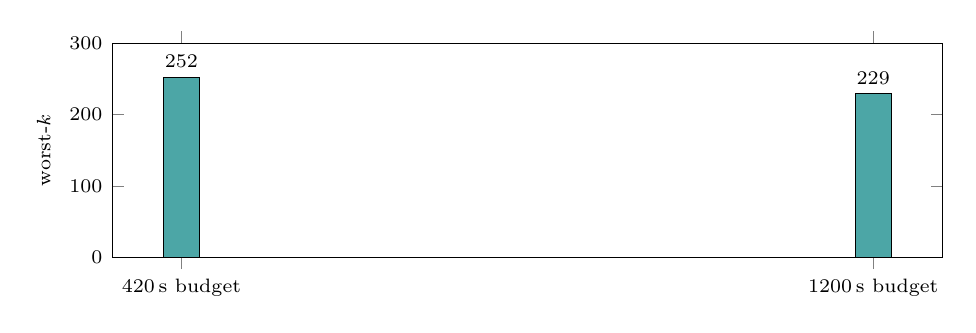
\begin{tikzpicture}
        \begin{axis}[width=\linewidth, height=4.3cm,
            ybar, bar width=13pt,
            symbolic x coords={420s,1200s},
            xtick=data, ymin=0, ymax=300,
            ylabel={worst-$k$}, ylabel style={font=\scriptsize},
            xticklabels={420\,s budget,1200\,s budget},
            nodes near coords, every node near coord/.append style={font=\scriptsize},
            tick label style={font=\scriptsize}]
          \addplot[fill=teal!70] coordinates {(420s,252) (1200s,229)};
        \end{axis}
      \end{tikzpicture}\\[-2pt]
      \footnotesize
      420\,s budget $\to$ finished in \textbf{381\,s}, \textbf{all 9 valid}.\\
      More budget $\to$ lower $k$; the hard graphs soak up the banked time.
    \end{column}
  \end{columns}
\end{frame}

% ---------------------------------------------------------------
\begin{frame}{One Folder, One Click}
  Wired straight into the dashboard --- a \textbf{Batch / Orchestrator} toggle in the
  run-control panel:
  \medskip
  \centering
  \begin{tikzpicture}[font=\small, node distance=0.55cm,
      step/.style={draw, rounded corners=3pt, minimum height=0.95cm,
                   minimum width=2.35cm, align=center}]
    \node[step, fill=muted!15] (f) {\textbf{Pick folder}\\{\scriptsize of graphs}};
    \node[step, fill=accent!15, right=of f] (s) {\textbf{Scan}\\{\scriptsize preview graphs}};
    \node[step, fill=teal!18, right=of s] (r) {\textbf{Scan \& Run}\\{\scriptsize auto-start}};
    \node[step, fill=warm!15, right=of r] (m) {\textbf{Live monitor}\\{\scriptsize log + $k$ table}};
    \draw[->, thick] (f) -- (s);
    \draw[->, thick] (s) -- (r);
    \draw[->, thick] (r) -- (m);
  \end{tikzpicture}
  \medskip
  \begin{columns}[T]
    \begin{column}{0.5\textwidth}
      \begin{itemize}
        \item Type the graph folder $\to$ \texttt{Scan} lists every valid graph found.
        \item \texttt{Scan \& Run} launches the orchestrator on that folder --- no
              other setup.
      \end{itemize}
    \end{column}
    \begin{column}{0.5\textwidth}
      \begin{itemize}
        \item Live log + per-graph \texttt{k\,/\,leases\,/\,valid} stream while it runs.
        \item Submissions land in \texttt{submission/}, keeping the \emph{original}
              file names.
      \end{itemize}
    \end{column}
  \end{columns}
  \medskip
  \centering
  \small\textcolor{teal}{\textbf{Analyse $\to$ allocate $\to$ half-share $\to$ submit --- inside the budget, hands-off.}}
\end{frame}
